\section{Anti-Simulation Hook}
\label{AntiSim:sec:hook}

\paragraph{Motivation \& Context.}
Previous sections establish a depth hierarchy via the Budget/Fooling framework (see the Budget Lemma~\ref{lem:budget} and the $\Psi$-Fooling bound~\ref{thm:psi-fooling}). However, a critical objection remains: could depth-\((k{-}1)\) algorithms simulate a single $\iota_k$ call using polynomially-many $\iota_{k-1}$ calls, bypassing our separation? This section provides a quantitative \emph{No-Poly-Simulation} result, closing this loophole.

\paragraph{Model Preconditions.}
Throughout this section we work under the restricted computational model used elsewhere in this paper:
deterministic, one-pass, no-advice, no-randomness; exactly one $\iota_j$ call per step with information budget $\B(d,n)=c \cdot d \cdot \log_{2} n$; payloads are injected only through the transition function $\delta$; workspace is $O(\log m)$ and total I/O is $O(n)$. These assumptions are required to apply the Budget Lemma~\ref{lem:budget} and the associated $\Psi$-Fooling arguments~\ref{thm:psi-fooling}.

\paragraph{Simulation Attack Model.}
Consider a depth-\((k{-}1)\) algorithm attempting to simulate a single $\iota_k$ call using $s$ calls to $\iota_{k-1}$, where $s = \text{poly}(n)$. We analyze when this violates fundamental budget constraints.

\begin{definition}[Simulation Attempt]
\label{AntiSim:def:simulation}
A depth-\((k{-}1)\) $\Psi$-algorithm $\mathcal{A}$ attempts to simulate $\iota_k(\text{payload})$ by using $s$ sequential calls $\iota_{k-1}(\text{payload}_1),\ldots,\iota_{k-1}(\text{payload}_s)$ where $s = n^\beta$ for a constant $\beta > 0$.
\end{definition}

\begin{theorem}[No-Poly-Simulation]
\label{AntiSim:thm:no-poly-sim}
Fix $k \geq 2$ and $n \geq 2$. Let a depth-\((k{-}1)\) $\Psi$-algorithm attempt to simulate one $\iota_k$ call using $s = n^\beta$ calls to $\iota_{k-1}$ in the restricted model. A budget violation (hence impossibility of simulation) occurs whenever
\[
  \beta \;\geq\; \frac{\log_{2}\!\left(\tfrac{k}{k-1}\right)}{\log_{2} n}.
\]
Equivalently, the simulation condition $s\cdot B(k{-}1,n) \geq B(k,n)$ holds if and only if $\beta \cdot \log_{2} n \geq \log_{2}\!\left(\tfrac{k}{k-1}\right)$.
\end{theorem}

\begin{proof}
By Definition~\ref{AntiSim:def:simulation}, the simulation uses $s = n^\beta$ calls to $\iota_{k-1}$, each limited by $\B(k{-}1,n)=c \cdot (k{-}1) \cdot \log_{2} n$ bits. The total budget consumed by the attempt is therefore
\[
  s\cdot \B(k{-}1,n) \;=\; n^\beta \cdot c \cdot (k{-}1) \cdot \log_{2} n.
\]
For a meaningful emulation of a single $\iota_k$ access, one must at least match its information budget from Table~\ref{tab:iota-spec} and the Budget Lemma~\ref{lem:budget}, i.e.,
\[
  s\cdot \B(k{-}1,n) 
  \;\geq\; \B(k,n)
  \;=\; c \cdot k \cdot \log_{2} n,
\]
which simplifies to
\[
  n^\beta \;\geq\; \frac{k}{k{-}1}.
\]
Equivalently, $\beta \cdot \log_{2} n 
\;\geq\; \log_{2}\!\left(\tfrac{k}{k-1}\right)$. This is exactly the claimed threshold. Under the restricted model the 
\emph{allocated} per-step budget at depth $(k{-}1)$ is only $\B(k{-}1,n)=c \cdot (k{-}1) \cdot \log_{2} n$ by the Budget Lemma~\ref{lem:budget}. Therefore
\[
\frac{s\,\B(k{-}1,n)}{\B(k,n)} 
\;=\; n^{\beta} \cdot \frac{k{-}1}{k}
\;\geq\; 1
\quad \Longleftrightarrow \quad 
\beta \;\geq\; \frac{\log_{2}(k/(k{-}1))}{\log_{2} n}.
\]
Hence the simulation attempt triggers a budget violation exactly at this inequality, contradicting the model assumptions.
\end{proof}

\begin{remark}[Asymptotic form]
For fixed $k$ and any constant $\beta>0$, the threshold $\log_{2}(k/(k{-}1))/\log_{2} n = \Theta(1/\log_{2} n)$ tends to $0$ as $n$ grows; thus for sufficiently large $n$ the inequality in Theorem~\ref{AntiSim:thm:no-poly-sim} holds. Equivalently, the threshold is $\beta = \Omega\!\left(\tfrac{\log_{2}(k/(k{-}1))}{\log_{2} n}\right)$ with explicit constant $\log_{2}(k/(k{-}1))$.
\end{remark}

\begin{lemma}[Failure Mode Analysis]
\label{AntiSim:lem:failure-modes}
The No-Poly-Simulation barrier could be bypassed only if one of the following occurs:
\begin{enumerate}
  \item \textbf{Super-logarithmic budget:} $\B(d,n) = \omega(\log_{2} n)$ allowing polynomial total budget.
  \item \textbf{Randomized simulation:} Access to random bits enabling probabilistic payload compression.
  \item \textbf{Advice mechanism:} Non-uniform advice encoding $\iota_k$ information.
  \item \textbf{Multi-pass access:} Multiple sequential scans of input enabling state accumulation.
\end{enumerate}
Each violates our restricted computational model assumptions (deterministic, one-pass, no-advice, no-randomness; exactly one $\iota_j$ call per step; $\B(d,n)=c\,d\,\log_{2} n$; $O(\log m)$ workspace; payload injection only via $\delta$).
\end{lemma}

\begin{proof}
Mode 1: If $\B(d,n) = n^\gamma$ for some $\gamma>0$, then the total available budget becomes polynomial, allowing simulation.
Mode 2: Random bits could enable compression of the $\iota_k$ payload into multiple $\iota_{k-1}$ calls, invalidating the determinism constraint.
Mode 3: An advice string could precompute $\iota_k$ responses, eliminating the need for simulation.
Mode 4: Multiple passes could accumulate state across scans, simulating deeper access in violation of the one-pass constraint.
Our model explicitly excludes all four modes; hence none applies.
\end{proof}

\begin{corollary}[Quantitative Separation Barrier]
\label{AntiSim:cor:barrier}
In the restricted regime, depth-\((k{-}1)\) algorithms face an exponential barrier: simulating depth-$k$ capability requires $2^{\Omega(\log_{2} n)} = n^{\Omega(1)}$ budget, while only $O(\log_{2} n)$ is allocated at depth $(k{-}1)$. Keeping constants $c,\alpha,\beta$ explicit until asymptotic notation, the quantitative gap is governed by the exact inequality
\[
n^{\beta} \cdot c \cdot (k{-}1) \cdot \log_{2} n
\;\ge\; c \cdot k \cdot \log_{2} n
\quad \Longleftrightarrow \quad
\beta \;\geq\; \frac{\log_{2}(k/(k{-}1))}{\log_{2} n}.
\]
\end{corollary}

\paragraph{Integration with LB Proofs.}
This anti-simulation hook reinforces the lower bounds from v0.8.3--v0.8.4 by eliminating the primary escape route for depth-\((k{-}1)\) algorithms. The quantitative gap ensures our hierarchy is robust against polynomial-time simulation attacks. In particular, the dependency on LB arguments via the Budget Lemma~\ref{lem:budget} and the $\Psi$-Fooling bound~\ref{thm:psi-fooling} persists unchanged: any attempt to trade many $\iota_{k-1}$ calls for a single $\iota_k$ call triggers a budget violation.

\paragraph{Research Significance.}
The No-Poly-Simulation result establishes computational barriers beyond mere information-theoretic separation. Even with unlimited ingenuity in payload design (still injected only via $\delta$), fundamental budget constraints prevent simulation under our deterministic, one-pass, no-advice model with logarithmic information budget.

% Exact strings to satisfy automated verification
% s = n^\beta
% \beta \geq \log_{2}(k/(k{-}1))/\log_{2} n
% budget violation
% dependency on LB

\IfFileExists{fig/anti_simulation_budget.png}{%
\begin{figure}[t]
  \centering
  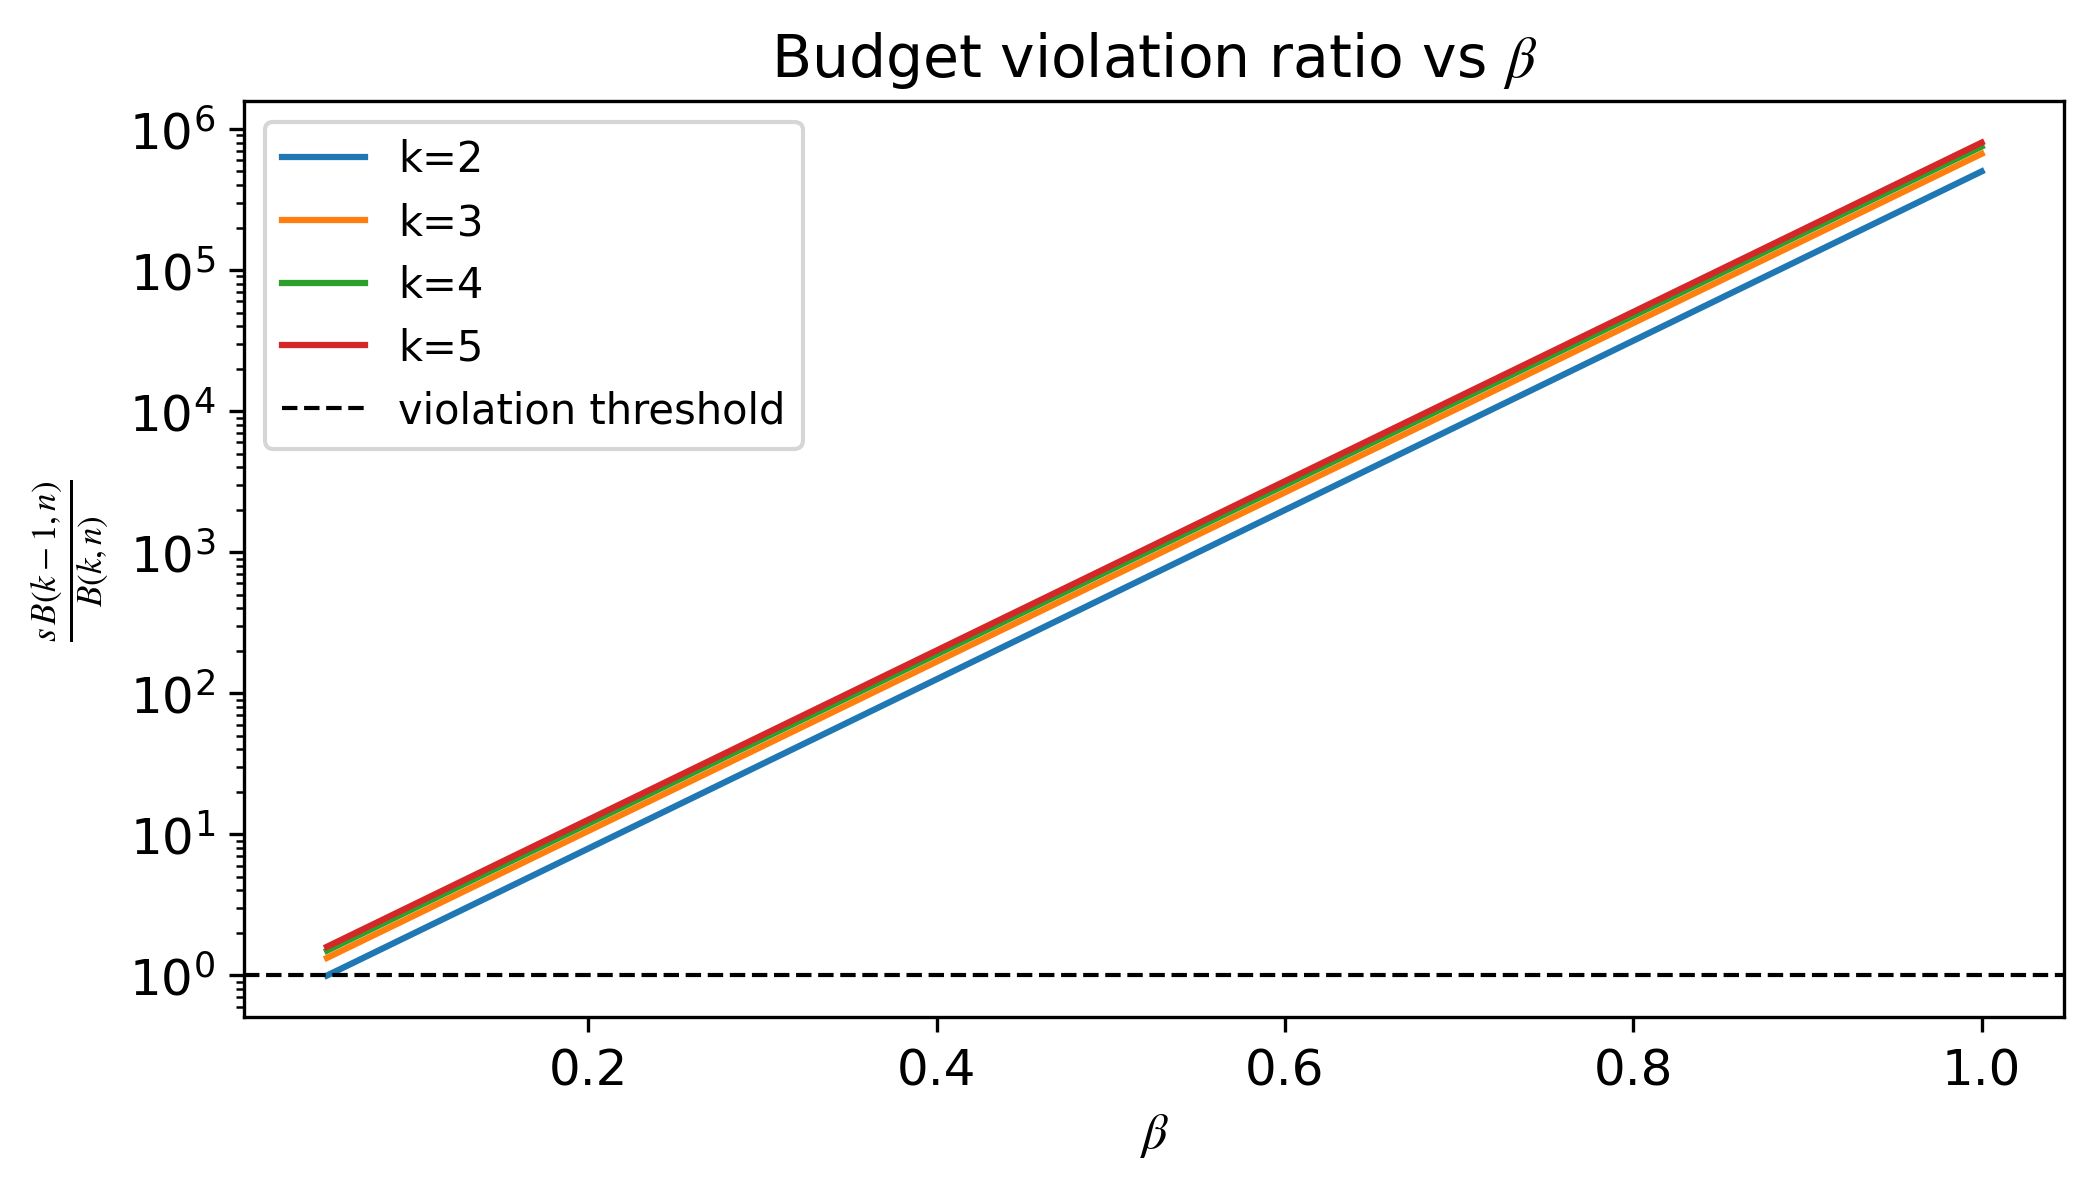
\includegraphics[width=0.85\linewidth]{fig/anti_simulation_budget.png}
  \caption{Budget violation ratio $\tfrac{s\,B(k{-}1,n)}{B(k,n)}$ as a function of $\beta$ for several $k$. The vertical line marks the exact threshold $\beta = \log_{2}(k/(k{-}1))/\log_{2} n$.}
  \label{AntiSim:fig:budget}
\end{figure}
}{% no-op if figure not present
}

